% !TEX root = 20230505_SHTSymposium.Presentation.tex

\title[MikroCT \& Histologie]{Was ist MikroCT und bringt das etwas Neues für die Histologie?}
\author{David Haberthür}
\date{5. Mai 2023 | Symposium Schweizerische Gesellschaft für Histologie-Technik}

\usetheme{UniBern}

%\includeonlyframes{current}
%then....
%\begin{frame}[label=current]
%\end{frame}

% Some often used abbreviations/commands
\newcommand{\everyframe}{1}% use only every nth frame for the animations
\newcommand{\imwidth}{\linewidth}% set global image width
\newcommand{\imheight}{0.618\paperheight}% set global image height
\newlength\imagewidth% needed for scalebars
\newlength\imagescale% needed for scalebars
\newcommand{\uct}{{\textmu}CT\xspace}% make our life easier
\newcommand{\eg}{e.\,g.\xspace}%
\newcommand{\ie}{i.\,e.\xspace}%

\usepackage[ngerman]{babel}
\usepackage[backend=biber,
	style=numeric,
	url=false,
	isbn=true,
	maxnames=1,
	sorting=none]{biblatex}
\addbibresource{../../Documents/library.bib}% FastSSD, Windows or Mac works (on Linux/FastSSD we generated a 'Document' folder at the correct level and `ln -s ~/P/Documents/library.bib .` to it)
\usepackage{standalone}
\usepackage{tikz}
	\usetikzlibrary{spy}
	\tikzset{shadowed/.style={preaction={transform canvas={shift={(1pt,-1pt)}},draw=ubRed}}}
\usepackage{shadowtext}% for the shadowed scalebar
	\shadowoffset{1pt}
	\shadowcolor{ubRed}
\usepackage{pgfplots}
	\pgfplotsset{compat=newest}
\usepackage[detect-all=true,
	range-phrase=--,
	range-units=single,
	per-mode=symbol,
	per-symbol=/]{siunitx}
\usepackage{microtype}
\usepackage[absolute,overlay]{textpos}%for the \source{} command
\usepackage[missing=main]{gitinfo2}% GitHub Actions don't pull in the commit hash, so we force the footer some lines down.
\usepackage{xspace}
\usepackage{ccicons}
\usepackage[version=4]{mhchem}
\usepackage{animate}
\usepackage{fontawesome5}
\usepackage{csquotes}
\usepackage{listings}
	\lstset{frame=single,
		%backgroundcolor = \color{lightgray},
		basicstyle=\tiny\ttfamily
		}
\usepackage{pgfplotstable}
\usepackage{booktabs}
\usepackage{colortbl}
\usepackage{multirow}
\usepackage{lipsum}%for alignment testing
\usepackage{mathastext}

% Define complementary colors to ubRed
\definecolor{ubRedComplementary1}{HTML}{00a1e6}
\definecolor{ubRedComplementary2}{HTML}{00e645}

% change tikz font to slide font
% https://tex.stackexchange.com/a/33329/828
\usepackage[eulergreek]{sansmath}
	\pgfplotsset{tick label style = {font=\sansmath\sffamily},
		every axis label = {font=\sansmath\sffamily},
		legend style = {font=\sansmath\sffamily},
		label style = {font=\sansmath\sffamily}
		}

% Globally thicker lines in with tikz
% https://tex.stackexchange.com/a/206769/828
\tikzset{every picture/.style={thick}}

% Acknowledge images just below them
% Based on https://tex.stackexchange.com/a/282637/828
\newcommand{\source}[2]{%
	% Print out (short) link under image, with small text
	\raisebox{-1.618ex}{%
		\makebox[0pt][r]{%
			\tiny\href{http://#1}{#1} #2%
			}%
		}%
	}%
\newcommand{\sourcecite}[2]{%
	% Cite (an image from) a reference
	\raisebox{-1.618ex}{%
		\makebox[0pt][r]{%
			\tiny From \cite{#1}, #2%
			}%
		}%
	}%
\newcommand{\sourcelink}[3]{%
	% Make the source command an \href{link}{text}
	\raisebox{-1.618ex}{%
		\makebox[0pt][r]{%
			\tiny\href{http://#1}{#2}, #3%
			}%
		}%
	}%

% Define us a custom footer *with* progress bar, based on https://tex.stackexchange.com/a/59749/828
\makeatletter
\def\progressbar@progressbar{}% the progress bar
\newcount\progressbar@tmpcounta% auxiliary counter
\newcount\progressbar@tmpcountb% auxiliary counter
\newdimen\progressbar@pbht%progressbar height
\newdimen\progressbar@pbwd%progressbar width
\newdimen\progressbar@rcircle% radius for the circle
\newdimen\progressbar@tmpdim% auxiliary dimension
\progressbar@pbwd=0.85\linewidth%
\progressbar@rcircle=1.5pt%
\def\progressbar@progressbar{%
	\progressbar@tmpcounta=\insertframenumber%
	\progressbar@tmpcountb=\inserttotalframenumber%
	\progressbar@tmpdim=\progressbar@pbwd%
	\multiply\progressbar@tmpdim by \progressbar@tmpcounta%
	\divide\progressbar@tmpdim by \progressbar@tmpcountb%
	\par%
		\begin{tikzpicture}%
			\draw[ubGrey] (0,0) -- ++ (\progressbar@pbwd,0);%
			\draw[draw=ubRed,fill=ubGrey] (\the\dimexpr\progressbar@tmpdim-\progressbar@rcircle\relax,.5\progressbar@pbht) circle (\progressbar@rcircle);%
		\end{tikzpicture}%
		\hfill%
		\mode<beamer>{bit.ly/SHTuCT\xspace|\xspace v.\xspace\href{https://github.com/habi/Talk.2023.SHTSymposium/commit/\gitHash}{\gitAbbrevHash}\xspace|\xspace\insertframenumber/\inserttotalframenumber}%
		\mode<handout>{bit.ly/SHTuCT\xspace|\xspace\today\xspace|\xspace\insertframenumber/\inserttotalframenumber}%
}
\addtobeamertemplate{footline}{}%
{%
	\begin{beamercolorbox}[wd=\paperwidth,center]{white}%
		\progressbar@progressbar%
	\end{beamercolorbox}%
}%
\makeatother

% Format bibliography for beamer
% http://tex.stackexchange.com/a/10686/828
\renewbibmacro{in:}{}
% http://tex.stackexchange.com/a/13076/828
\AtEveryBibitem{%
	\clearfield{journaltitle}
	\clearfield{pages}
	\clearfield{volume}
	\clearfield{number}
	\clearname{editor}
	\clearfield{issn}
	\clearfield{year}
}
% No parentheses around the (now empty) year: https://tex.stackexchange.com/a/147537/828
\renewcommand{\bibopenparen}{\addcomma\addspace}
\renewcommand{\bibcloseparen}{\addcomma\addspace}

% Redefine \footcite based on https://tex.stackexchange.com/a/453528/828
\DeclareCiteCommand{\footcite}[\mkbibfootnote]{%
	\usebibmacro{prenote}}{%
		\printnames[family-given]{labelname}%
		\newunit%
		\printfield{doi}%
		\newunit%
		\printlabeldateextra%
	}{\addsemicolon\space}{%
		\usebibmacro{postnote}%
	}%

% References as footnotes at the bottom of the slides
% https://tex.stackexchange.com/a/368760/828
\makeatletter
\renewcommand\@makefnmark{\xspace\hbox{\usebeamercolor[fg]{footnote mark}\usebeamerfont*{footnote mark}[\@thefnmark]}}
\renewcommand\@makefntext[1]{\tiny{\usebeamercolor[fg]{footnote mark}\usebeamerfont*{footnote mark}[\@thefnmark]}\enspace\usebeamerfont*{footnote} #1}
\makeatother

% Show current section at begin of sections, but only in presentation mode
\mode<beamer>{%
	\AtBeginSection[]{%
		\begin{frame}{Contents}
			\tableofcontents[currentsection,currentsubsection,hideothersubsections]
		\end{frame}
	}
}

% Slide transiton
%\addtobeamertemplate{background canvas}{\transfade[duration=0.5]}{}

% open in fullscreen
%\hypersetup{pdfpagemode=FullScreen}

% Move the text down a bit
% THIS IS A BIG HACK, IT SHOULD BE FIXED IN THE TEMPLATE
\addtobeamertemplate{frametitle}{}{\vspace*{0.75em}}

\begin{document}
% No footline on the title page
% http://tex.stackexchange.com/a/18829/828 helps us to achieve that
{%
	\setbeamertemplate{footline}{}%
	\begin{frame}%
		\maketitle
	\end{frame}%
}

%% Alignment frames to test the ugly text-block-movement hack above
%\begin{frame}[label=current]{Alignment frame}
%	\begin{tikzpicture}%
%		\def\cut{2}%
%		\draw [|-|,ultra thick] (0,\cut) -- (0,\textheight-\cut);%
%		\draw [<->,ultra thick] (0.5\textwidth,\cut) -- (0.5\textwidth,\textheight-\cut);%
%		\draw [|-|,ultra thick] (\textwidth,\cut) -- (\textwidth,\textheight-\cut);%
%	\end{tikzpicture}%
%\end{frame}
%
%\begin{frame}[allowframebreaks,label=current]{Alignment frame II}
%	\lipsum[1-3]
%\end{frame}

\begin{frame}
	\frametitle{Grüessech mitenang!}
	\begin{itemize}
		\item David Haberthür
		\begin{itemize}
			\item Physiker
			\item \href{https://boris.unibe.ch/2619/}{Doktorarbeit über höchstaufgelöste tomographische Bildgebung in der Lunge} am Institut für Anatomie der Universität Bern
			\item Post-Doc I: Tomographische Bildgebung von Allerlei an \href{https://www.psi.ch/sls/tomcat/}{TOMCAT} am \href{https://www.psi.ch/}{Paul Scherrer Institut}
			  und Mitarbeit am \href{http://globaldiagnostix.org}{GlobalDiagnostiX}-Projekt
			\item Post-Doc II \& Gegenwart: Tomographische Bildgebung von biomedizinischen Dingen in der \href{https://www.ana.unibe.ch/forschung/mikroct/research/}{\uct-Gruppe} am Institut für Anatomie der Universität Bern
		\end{itemize}
	\end{itemize}
\end{frame}

\begin{frame}
	\frametitle{\uct-Gruppe}
	\begin{columns}
		\begin{column}{0.61\linewidth}
			\begin{itemize}
				\item microangioCT~\cite{Hlushchuk2018}
				\begin{itemize}
					\item Angiogenese: Herz, Muskulatur~\cite{Nording2021} und Knochen
					\item Gefässe: (Mäuse) Gehirn~\cite{Hlushchuk2020}, (humane) Nerven~\cite{Wuthrich2020}, (human) Hautgewebe~\cite{Zubler2021} und Tumore
				\end{itemize}
				\item Zebrafish Muskulatur und Kiemen~\cite{MesserliAaldijk2020}
				\item Erkennung und Klassierung von (Lungen) Tumoren und Metastasen~\cite{Trappetti2021}
				\item Zusammenarbeit mit NMBE~\cite{Bochud2021} und Wissenschaftler:innen an der Universität Bern~\cite{Halm2021,Haberthuer2023}
			\end{itemize}
		\end{column}
		\begin{column}{0.37\linewidth}
			\centering
			\includegraphics<1|handout:0>[width=\imwidth]{./images/1172}%
			\only<1|handout:0>{\source{brukersupport.com}{}}
			\includegraphics<2>[width=\imwidth]{./images/1272}%
			\only<2>{\source{bruker.com/skyscan1272}{}}
			\includegraphics<3|handout:0>[width=\imwidth]{./images/2214}%
			\only<3|handout:0>{\source{bruker.com/skyscan2214}{}}
		\end{column}
	\end{columns}
\end{frame}

\begin{frame}{Inhalt}
	\tableofcontents
\end{frame}

\section{Bildgebung}
\begin{frame}
	\frametitle{Wellenlänge und Grössenordnungen}
	\centering
	\only<1|handout:1>{%
		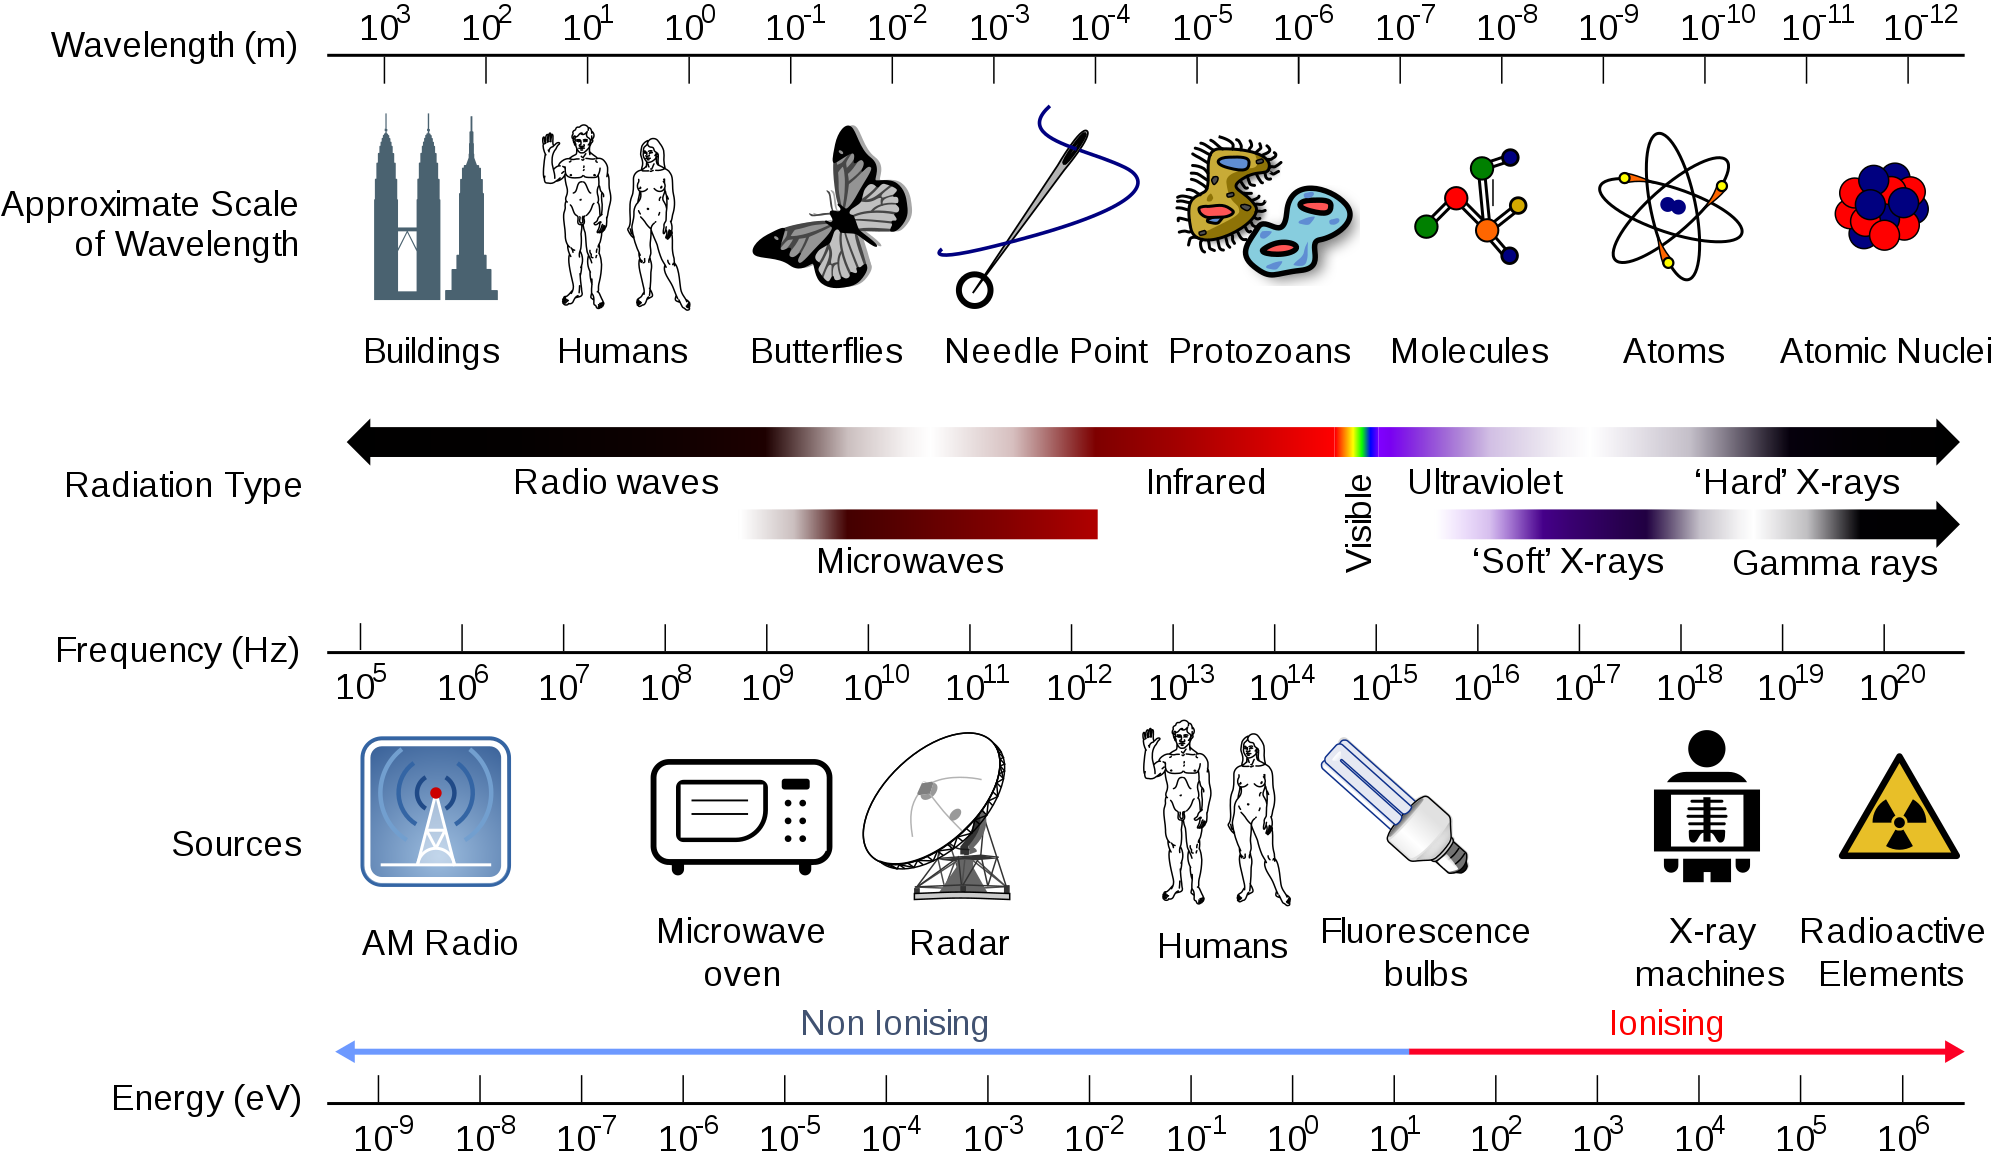
\includegraphics[height=\imheight]{./images/2000px-Electromagnetic_spectrum_with_sources}%
		\source{w.wiki/7fz}{\ccbysa}%
		}%
	\only<2|handout:2>{%
		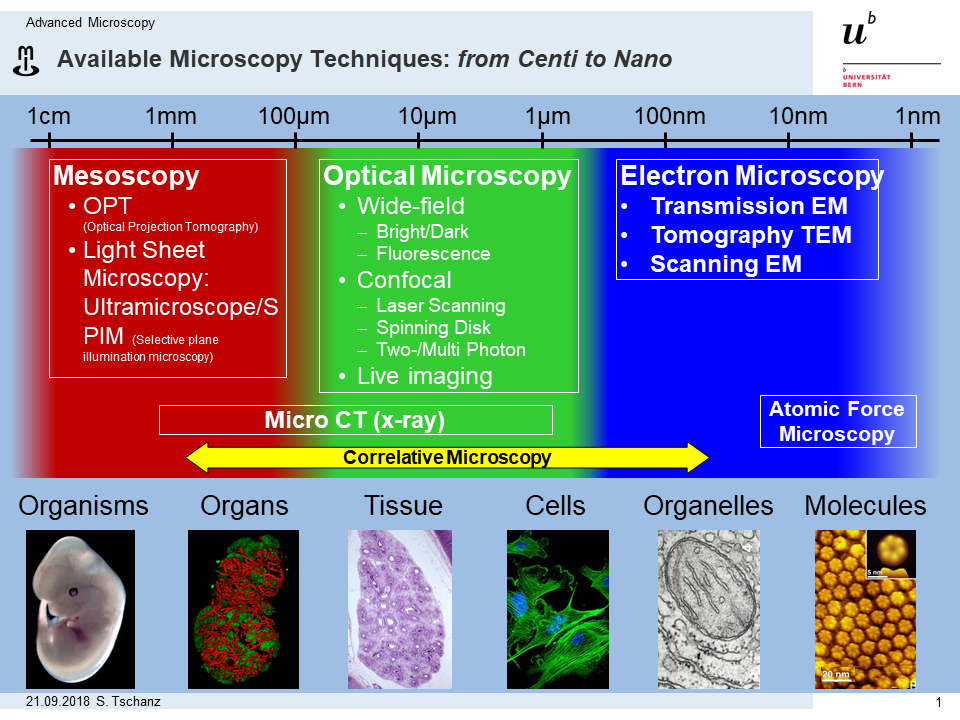
\includegraphics[height=\imheight]{./images/MIC-AM_techniques}%
		\sourcelink{https://anatomie.unibe.ch/tschanz}{Stefan Tschanz}{, mit Erlaubnis}%
		}
\end{frame}

\mode<beamer>{\begin{frame}[shrink=20]}
\mode<handout>{\begin{frame}[allowframebreaks]}
	\frametitle{Literatur}
	\mode<beamer>{\renewcommand*{\bibfont}{\tiny}}
	\mode<handout>{\renewcommand*{\bibfont}{\scriptsize}}
	\setbeamertemplate{bibliography item}{\insertbiblabel}
	\printbibliography
\end{frame}

\end{document}
